% =====================================================================
%  Informe TP N.º 1 - I206 Inferencia y Estimación - UdeSA
%  COMPLETAR antes de entregar: número de grupo, legajos y profesores
%  (ver los comandos \grupo, \legajo... y \profesores más abajo).
%  Compilar desde esta carpeta: las figuras se leen de ../figures/
% =====================================================================
\documentclass[11pt,a4paper]{article}

\usepackage[utf8]{inputenc}
\usepackage[T1]{fontenc}
\usepackage{lmodern}
\usepackage[spanish,es-tabla,es-nodecimaldot,es-noquoting]{babel}
\usepackage{amsmath,amssymb}
\usepackage{dsfont}
\usepackage{graphicx}
\usepackage[a4paper,margin=2.2cm]{geometry}
\usepackage{booktabs}
\usepackage{float}
\usepackage[font=small,labelfont=bf,skip=4pt]{caption}
\usepackage{enumitem}
\usepackage{fancyhdr}
\usepackage{microtype}
\usepackage[hidelinks]{hyperref}

\graphicspath{{../figures/}}

% ---------------------- Datos para completar ----------------------
\newcommand{\grupo}{1}
\newcommand{\legajoAlsina}{370833}
\newcommand{\legajoBunge}{370842}
\newcommand{\legajoDietrich}{XXXXX}
\newcommand{\profesores}{Copa, Débora; Carducci, Leonardo; García Gulisano Pau}
% ------------------------------------------------------------------

\newcommand{\E}{\mathbb{E}}
\newcommand{\Prob}{\mathbb{P}}
\newcommand{\ind}{\mathds{1}}
\newcommand{\acc}{\emph{accuracy}}

\setlength{\parskip}{0.25em}
\setlist{itemsep=0.15em, topsep=0.25em}
\setlength{\textfloatsep}{10pt plus 2pt minus 2pt}
\setlength{\floatsep}{8pt plus 2pt minus 2pt}

\pagestyle{fancy}
\fancyhf{}
\lhead{Inferencia y Estimación}
\rhead{Trabajo Práctico N.\textsuperscript{o} 1 -- Grupo \grupo}
\cfoot{\thepage}
\setlength{\headheight}{14pt}

\begin{document}

% =====================================================================
%  Carátula
% =====================================================================
\begin{titlepage}
  \centering
  \vspace*{1cm}
  {\Large Universidad de San Andrés\par}
  \vspace{0.3cm}
  {\large Ingeniería en Inteligencia Artificial\par}
  \vspace{0.3cm}
  {\large I206 -- Inferencia y Estimación\par}
  \vspace{3cm}
  {\Huge\bfseries Trabajo Práctico N.\textsuperscript{o} 1\par}
  \vspace{0.8cm}
  {\LARGE Análisis de Componentes Principales\\[0.2cm] y Simulación Monte Carlo\par}
  \vspace{0.5cm}
  {\large Clasificación de radiografías de tórax (PneumoniaMNIST)\par}
  \vspace{3cm}
  {\large\bfseries Grupo \grupo\par}
  \vspace{0.5cm}
  {\large
  \begin{tabular}{l@{\hspace{1.5cm}}l}
    Bautista Alsina & Legajo \legajoAlsina \\[0.15cm]
    Santos Bunge    & Legajo \legajoBunge \\[0.15cm]
    Hans Dietrich   & Legajo \legajoDietrich \\
  \end{tabular}\par}
  \vspace{1.5cm}
  {\large Profesores: \profesores\par}
  \vfill
  {\large Primavera 2026\par}
\end{titlepage}

% =====================================================================
\section*{Resumen}
% =====================================================================
En este trabajo usamos el Análisis de Componentes Principales (PCA) para reducir la dimensión de
radiografías de tórax y evaluamos, con un clasificador de regresión logística, cuánta información útil se
conserva para distinguir pacientes sanos de pacientes con neumonía. Con las imágenes completas (16384
píxeles) el clasificador obtuvo un \acc{} de 0.818. Con solo 3 componentes principales se alcanzó el mismo
desempeño, y con 5 se llegó a 0.857. Luego estudiamos con simulaciones de Monte Carlo qué ocurre si las
imágenes de prueba se rotan 180° con probabilidad $p$. El \acc{} medio disminuye linealmente con $p$, y la
probabilidad de perder más de 0.1 de \acc{} es nula para $p \le 0.20$ y supera 0.97 para $p \ge 0.45$.
Finalmente, justificamos los estimadores utilizados con la Ley de los Grandes Números.

% =====================================================================
\section{Introducción}
% =====================================================================
Una radiografía digital de $128\times128$ píxeles puede verse como un vector de 16384 números, uno por
píxel. Trabajar con vectores tan grandes es costoso y, además, poco eficiente, porque gran parte de esos
valores son redundantes: los píxeles vecinos suelen parecerse y todas las radiografías comparten la forma
general del tórax. El Análisis de Componentes Principales (PCA) aprovecha esta redundancia. Busca
direcciones, formadas por combinaciones de píxeles, ordenadas según cuánta variabilidad de los datos
explica cada una, de modo que cada imagen puede describirse con sus primeras $K$ coordenadas. Para medir si
esa representación conserva la información importante, usamos un clasificador de regresión logística (LR)
que decide si una radiografía corresponde a un paciente sano o con neumonía, y comparamos su \acc{}
(proporción de aciertos) con y sin PCA.

En la segunda parte analizamos qué tan robusto es este sistema si algunas imágenes llegan rotadas 180°.
Como no se sabe de antemano cuáles llegarán rotadas, tratamos la situación como un experimento aleatorio y
la estudiamos con simulaciones de Monte Carlo, es decir, repitiendo el experimento muchas veces con sorteos
independientes y resumiendo los resultados. La Ley de los Grandes Números es la que justifica que esos
promedios se acerquen a los valores verdaderos.

Los objetivos del trabajo son: (i) obtener un desempeño de referencia con las imágenes completas;
(ii) implementar PCA mediante la descomposición en valores singulares y visualizar los datos en las dos
primeras componentes; (iii) analizar el \acc{} en función de $K$; (iv) estimar con Monte Carlo el \acc{}
medio, la probabilidad de superar una pérdida tolerable y la distribución del \acc{} bajo rotaciones
aleatorias; y (v) justificar teóricamente el estimador de probabilidad utilizado.

% =====================================================================
\section{Datos y metodología}
% =====================================================================
\paragraph{Datos.} Usamos imágenes de PneumoniaMNIST~\cite{medmnist} de $128\times128$ píxeles en escala de
grises, con etiqueta 0 (paciente sano, clase \emph{Normal}) o 1 (\emph{Neumonía}). El conjunto de
entrenamiento tiene 2428 imágenes (1214 de cada clase) y el de prueba, 468 (234 de cada clase). Como ambos
están balanceados, un clasificador que respondiera al azar obtendría un \acc{} de aproximadamente 0.5, que
tomamos como referencia mínima. Leímos las imágenes en el mismo orden que los archivos de etiquetas, para
que cada una quedara asociada a su etiqueta correcta. Luego transformamos cada imagen en un vector fila de
16384 valores y apilamos esos vectores, obteniendo $X_{\text{train}} \in \mathbb{R}^{2428\times16384}$ y
$X_{\text{test}} \in \mathbb{R}^{468\times16384}$.

\paragraph{PCA mediante SVD.} Calculamos la imagen media de entrenamiento, $\mu$, y la restamos a cada fila
para obtener la matriz centrada $X_c = X_{\text{train}} - \mu$. Luego calculamos su descomposición en
valores singulares (SVD) reducida, $X_c = U S V^T$~\cite{teoricas}. Las columnas $v_1, v_2, \dots$ de $V$
son las direcciones principales, ordenadas según los valores singulares $s_1 \ge s_2 \ge \dots$, y la
fracción de la varianza total que explica la componente $j$ es $s_j^2/\sum_i s_i^2$. Para conservar $K$
componentes formamos la matriz $V_K$ con las primeras $K$ columnas de $V$ y proyectamos cualquier conjunto
de imágenes como
\[ Z = (X - \mu)\,V_K , \]
donde cada fila de $Z$ contiene las $K$ coordenadas de una imagen. Las decisiones más importantes fueron:
\begin{itemize}
  \item \textbf{Usar SVD en lugar de la matriz de covarianza.} Las direcciones principales son los
        autovectores de $C = X_c^TX_c/(n-1)$, pero $C$ tendría $16384\times16384$ elementos (unos 2\,GB de
        memoria). Como $C = VS^2V^T/(n-1)$, la SVD entrega esos mismos autovectores trabajando directamente
        con los datos, sin construir $C$.
  \item \textbf{Calcular una sola SVD para todos los $K$.} La descomposición ya contiene todas las
        direcciones ordenadas, así que cambiar $K$ solo implica tomar más o menos columnas de $V$, sin
        repetir el cálculo más costoso.
  \item \textbf{Calcular $\mu$ y $V_K$ solo con el conjunto de entrenamiento.} El conjunto de prueba
        representa datos nuevos, por lo que no debe usarse en ninguna parte del entrenamiento, y PCA forma
        parte de esa etapa. Por eso las imágenes de prueba se centran con la media de entrenamiento y se
        proyectan con sus direcciones.
  \item \textbf{Usar la misma fórmula para ambos conjuntos.} Para las imágenes de entrenamiento se cumple
        $(X_{\text{train}}-\mu)V_K = U_KS_K$, pero esta igualdad no sirve para las de prueba, porque $U$
        corresponde solo al conjunto de entrenamiento. Por eso usamos siempre $Z=(X-\mu)V_K$, que vale para
        cualquier imagen.
\end{itemize}

\paragraph{Clasificador y métrica.} Usamos la regresión logística de \emph{scikit-learn}~\cite{sklearn} con
un máximo de 2000 iteraciones, para que el ajuste tenga pasos suficientes para converger, y dejamos el resto
de los parámetros en sus valores por defecto. No analizamos su funcionamiento interno~\cite{mahmood}, ya que
lo usamos solo como herramienta de comparación. Siempre entrenamos con el conjunto de entrenamiento y
medimos el \acc{} sobre las 468 imágenes de prueba. Cada acierto modifica el \acc{} en $1/468\approx0.002$,
así que una diferencia de 0.01 equivale a unas 5 imágenes. Tener en cuenta esta escala nos ayudó a no
sobreinterpretar diferencias pequeñas.

\paragraph{Organización del código.} El código está en dos cuadernos de Jupyter, uno por ejercicio
práctico. En el primero dividimos el trabajo en funciones cortas con una sola tarea cada una: leer imágenes
y etiquetas, vectorizarlas, entrenar y evaluar el clasificador, calcular PCA, proyectar y recorrer valores
de $K$. Esto nos permitió reutilizarlas en todos los incisos. El segundo cuaderno carga los datos y entrena
el modelo por su cuenta, de modo que puede ejecutarse de forma independiente. Ambos usan NumPy~\cite{numpy}
y guardan las figuras en una carpeta común.

% =====================================================================
\section{Ejercicio 1: PCA y clasificación}
% =====================================================================
\subsection{Clasificador con las imágenes completas}

Entrenamos la regresión logística con los 16384 píxeles de cada imagen (valores entre 0 y 255) y obtuvimos
un \acc{} de \textbf{0.818} (383 aciertos de 468), que usamos como línea de base. En este caso el modelo
ajusta un peso por píxel, es decir, 16384 parámetros, con solo 2428 imágenes de entrenamiento. Cuando hay
muchos más parámetros que ejemplos, el modelo puede aprender detalles propios de las imágenes de
entrenamiento que no se repiten en imágenes nuevas. Este fenómeno se conoce como \emph{sobreajuste} y lo
retomamos más adelante.

\subsection{Proyección sobre las dos primeras componentes}

La Figura~\ref{fig:scatter} muestra las imágenes de prueba proyectadas sobre las dos primeras componentes
calculadas con el conjunto de entrenamiento. Sobre la componente 1 (eje horizontal) ambas clases ocupan casi
todo el rango, por lo que esta coordenada sola no permite distinguirlas. Sobre la componente 2 (eje
vertical), en cambio, las imágenes normales tienden a tomar valores positivos y las de neumonía, negativos.
La separación no es perfecta: cerca de cero se mezclan puntos de ambas clases, por lo que cualquier frontera
recta va a cometer errores, lo que es coherente con el \acc{} de 0.803 obtenido con $K=2$. Los ejes llegan a
valores del orden de los miles porque en este cuaderno usamos los píxeles sin normalizar.

\subsection{Accuracy en función de la cantidad de componentes}

Para cada $K$ entre 1 y 300 proyectamos ambos conjuntos, entrenamos una regresión logística nueva (la
cantidad de entradas cambia con $K$) y medimos su \acc{}. Elegimos este rango porque muestra tanto el
comportamiento con muy pocas componentes como la tendencia para valores grandes de $K$. Los resultados se
presentan en la Figura~\ref{fig:acck} y en la Tabla~\ref{tab:acck}.

\begin{figure}[H]
  \centering
  \begin{minipage}[t]{0.47\textwidth}\vspace{0pt}
    \centering
    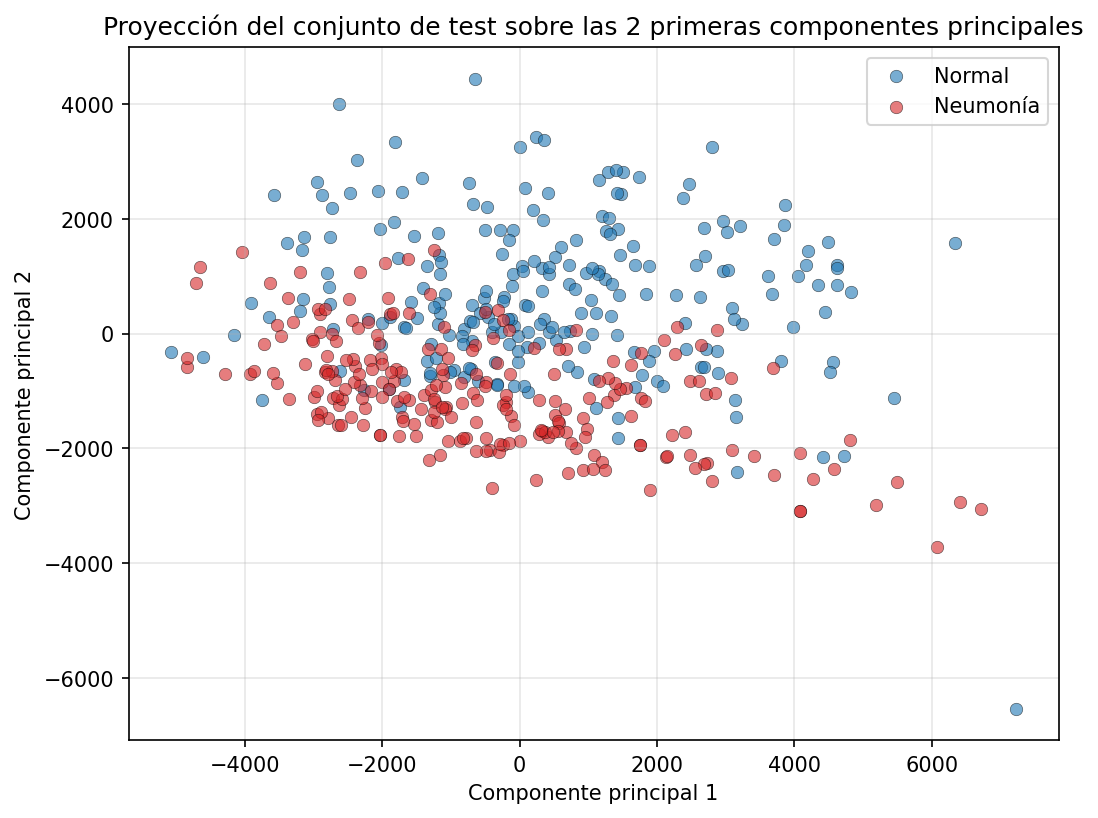
\includegraphics[height=5.6cm]{pca_scatter.png}
    \caption{Conjunto de prueba proyectado sobre las dos primeras componentes principales
             (azul: Normal; rojo: Neumonía).}
    \label{fig:scatter}
  \end{minipage}\hfill
  \begin{minipage}[t]{0.51\textwidth}\vspace{0pt}
    \centering
    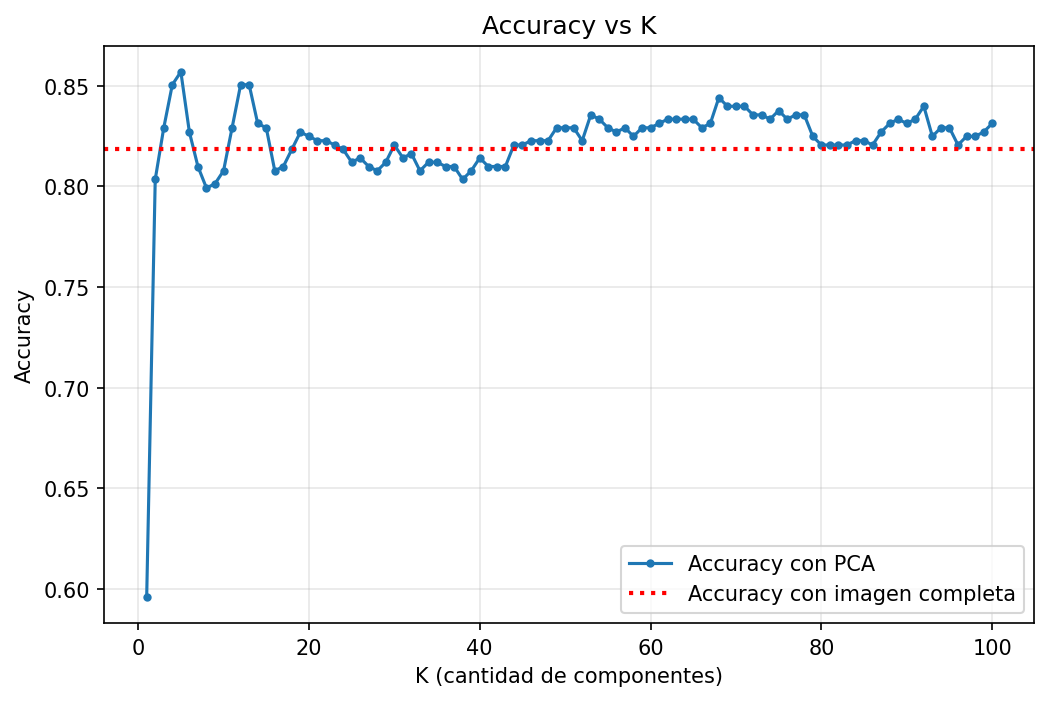
\includegraphics[height=5.6cm]{accuracy_vs_k.png}
    \caption{\emph{Accuracy} de PCA+LR en función de $K$ y \emph{accuracy} con la imagen completa
             (línea punteada).}
    \label{fig:acck}
  \end{minipage}
\end{figure}

\begin{table}[H]
  \centering
  \caption{Varianza explicada acumulada y \emph{accuracy} sobre el conjunto de prueba para algunos valores
           de $K$. Sin PCA, el \emph{accuracy} es 0.818.}
  \label{tab:acck}
  \small\setlength{\tabcolsep}{3pt}
  \begin{tabular}{lcccccccccc}
    \toprule
    $K$ & 1 & 2 & 3 & 5 & 10 & 20 & 50 & 100 & 200 & 300 \\
    \midrule
    Varianza acumulada & 28.3\,\% & 38.4\,\% & 44.7\,\% & 54.0\,\% & 66.0\,\% & 75.5\,\% & 83.9\,\% & 88.7\,\% & 93.1\,\% & 95.2\,\% \\
    \emph{Accuracy}    & 0.596 & 0.803 & 0.829 & \textbf{0.857} & 0.808 & 0.825 & 0.829 & 0.831 & 0.812 & 0.786 \\
    \bottomrule
  \end{tabular}
\end{table}

Con $K=1$ el \acc{} es 0.596, apenas mayor que el azar, lo que concuerda con que la primera componente no
separa las clases. Con $K=2$ sube a 0.803, gracias a la segunda componente. Con $K=3$ ya se supera la línea
de base (0.829), y con $K=5$ se alcanza el máximo del rango estudiado, 0.857 (401 aciertos). Es decir, con
solo 5 números por imagen el clasificador funciona mejor que con los 16384 píxeles. Entre $K\approx20$ y
$K\approx180$ la curva oscila entre 0.80 y 0.85 alrededor de la línea de base sin una tendencia de mejora,
y a partir de $K\approx190$ queda por debajo de ella y desciende de forma sostenida hasta 0.786 en $K=300$:
agregar componentes de baja varianza no aporta información útil y, con 2428 muestras de entrenamiento,
suma parámetros que terminan perjudicando la generalización. Las oscilaciones entre
valores cercanos de $K$, como el pico en $K=12$ y $K=13$, corresponden a diferencias de pocas imágenes (0.02
equivale a unas 9), por lo que no les dimos importancia individualmente.

Que pocas componentes superen a la imagen completa puede parecer contradictorio, ya que al proyectar se
descarta información. Una posible explicación es que lo descartado son sobre todo detalles de baja varianza
no relacionados con la enfermedad, y que un modelo con pocas entradas tiene muchos menos parámetros y, por
lo tanto, menos riesgo de sobreajuste. Así, la reducción de dimensión no solo ahorra cómputo, sino que
también puede ayudar al clasificador a generalizar.

\subsection{Análisis complementario: interpretación de las componentes}

Para entender \emph{por qué} alcanzan pocas componentes, hicimos tres análisis adicionales.

\paragraph{Componentes como imágenes.} Cada dirección $v_j$ tiene un peso por píxel, así que puede
graficarse como una imagen de $128\times128$ (Figura~\ref{fig:comp}; rojo: pesos positivos, azul:
negativos). El signo global de cada componente es arbitrario, por lo que lo que se interpreta es el
contraste entre zonas. La \textbf{PC1} (28.3\,\% de la varianza) tiene todos sus pesos del mismo signo, así
que mide básicamente el brillo total de la imagen: su correlación con el brillo medio es $-0.98$, y el signo
negativo solo refleja la elección arbitraria del signo. El brillo depende más de la exposición o del tamaño
del paciente que de la enfermedad, lo que explica el bajo \acc{} con $K=1$. La \textbf{PC2} (10.1\,\%) tiene
signos opuestos en los pulmones y en la periferia del tórax, así que mide qué tan claros se ven los pulmones
respecto del resto. Un pulmón sano se ve oscuro porque está lleno de aire, mientras que la neumonía produce
zonas opacas, y por eso esta componente separa las clases. Las \textbf{PC3 a PC6} reflejan otros patrones,
como el brillo de los pulmones en conjunto, el encuadre o asimetrías entre los lados, que no parecen estar
asociados a la clase.

\begin{figure}[H]
  \centering
  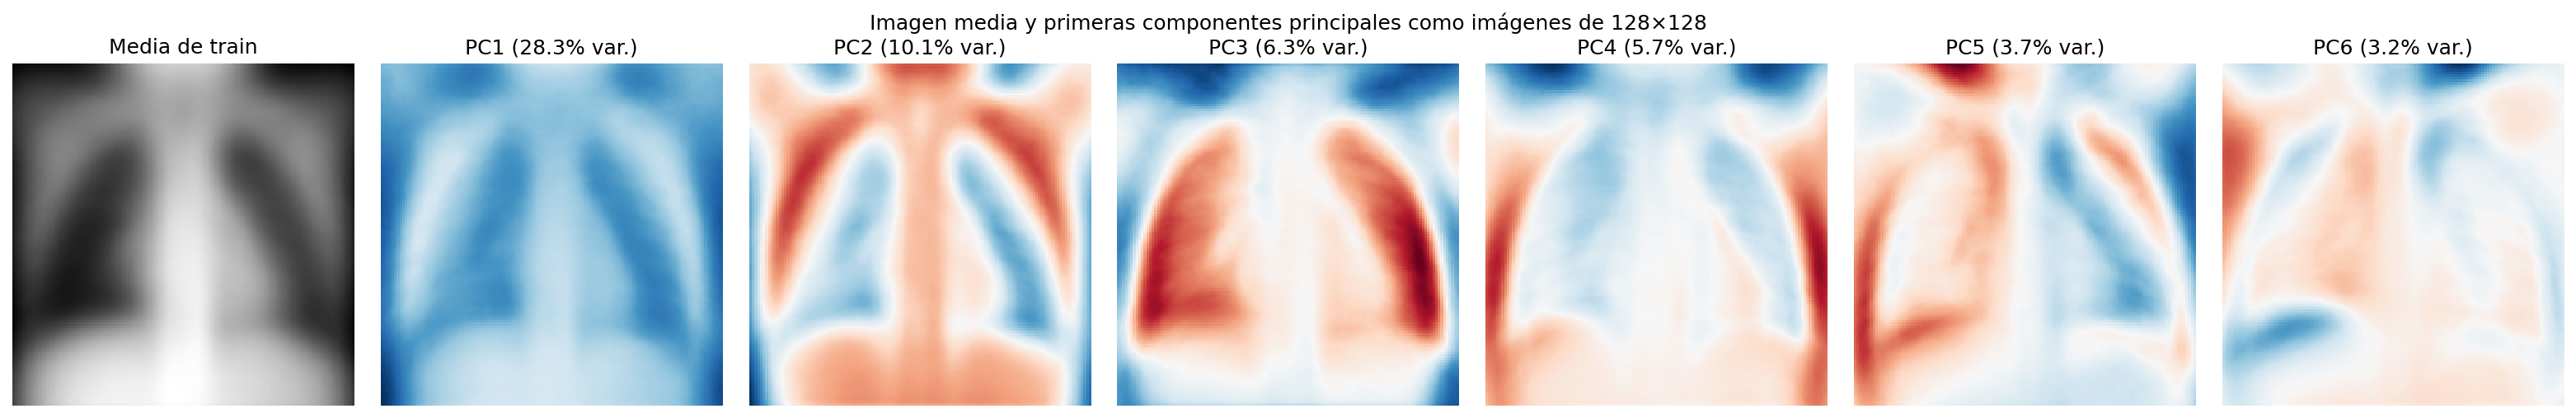
\includegraphics[width=\textwidth]{pca_componentes_imagenes.png}
  \caption{Imagen media de entrenamiento y primeras seis componentes principales vistas como imágenes.}
  \label{fig:comp}
\end{figure}

\paragraph{Varianza explicada.} La Figura~\ref{fig:var} superpone el \acc{} con la varianza acumulada. Un
criterio habitual es elegir $K$ de modo de conservar el 90\,\% de la varianza. Aquí eso requeriría 121
componentes, mientras que la línea de base se alcanza con $K=3$, que conserva solo el 44.7\,\% de la
varianza. Por lo tanto, para clasificar conviene elegir $K$ según el desempeño del clasificador y no solo
según la varianza conservada.

\begin{figure}[H]
  \centering
  \begin{minipage}[t]{0.57\textwidth}\vspace{0pt}
    \centering
    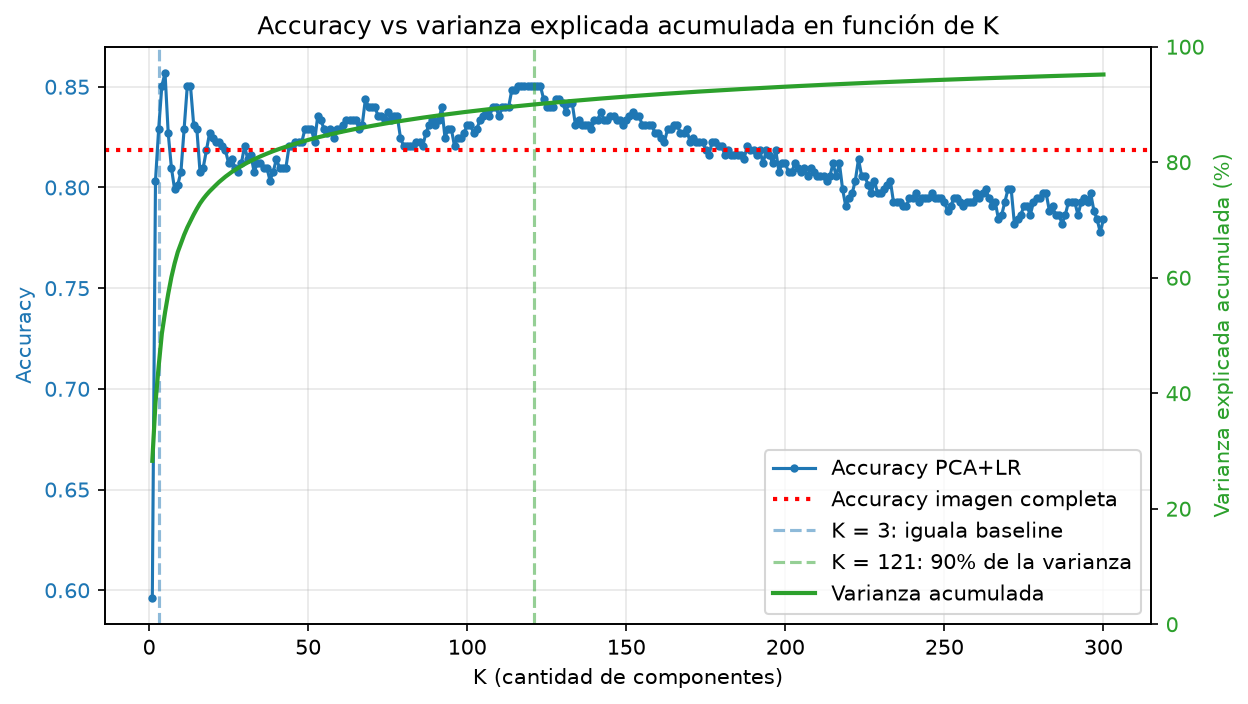
\includegraphics[width=\linewidth]{accuracy_vs_varianza.png}
    \caption{\emph{Accuracy} (eje izquierdo) y varianza explicada acumulada (eje derecho) en función de $K$.}
    \label{fig:var}
  \end{minipage}\hfill
  \begin{minipage}[t]{0.39\textwidth}\vspace{0pt}
    \centering
    \captionof{table}{Varianza, cociente de Fisher $F$ y \emph{accuracy} usando una sola coordenada.}
    \label{tab:fisher}
    \small
    \begin{tabular}{lccc}
      \toprule
      Comp. & Varianza & $F$ & \emph{Acc.} \\
      \midrule
      PC1 & 28.3\,\% & 0.232 & 0.596 \\
      PC2 & 10.1\,\% & \textbf{1.477} & \textbf{0.784} \\
      PC3 & 6.3\,\%  & 0.067 & 0.583 \\
      PC4 & 5.7\,\%  & 0.074 & 0.592 \\
      PC5 & 3.7\,\%  & 0.031 & 0.491 \\
      PC6 & 3.2\,\%  & 0.063 & 0.436 \\
      \bottomrule
    \end{tabular}
  \end{minipage}
\end{figure}

\paragraph{Separación por componente.} Para cuantificar cuánto separa cada componente por sí sola,
calculamos sobre el conjunto de entrenamiento el cociente de Fisher $F = (m_0-m_1)^2/(\sigma_0^2+\sigma_1^2)$,
donde $m_c$ y $\sigma_c^2$ son la media y la varianza de la coordenada en la clase $c$. El numerador mide la
distancia entre los centros de las clases y el denominador, su dispersión, de modo que un $F$ mayor indica
una mejor separación. También medimos el \acc{} de una regresión logística entrenada con esa única
coordenada. La Tabla~\ref{tab:fisher} confirma lo observado. La PC2 es la única componente que separa por sí
sola: su $F$ es más de seis veces el de la PC1 y al menos veinte veces el de las PC3 a PC6, y alcanza un
\acc{} de 0.784. En resumen, PCA ordena las direcciones por varianza sin mirar las etiquetas, así que la de
mayor varianza no tiene por qué ser la más útil para clasificar. En este problema funcionó bien porque la
opacidad pulmonar resultó ser la segunda fuente de variación más importante, pero eso no está garantizado en
otros casos.

% =====================================================================
\section{Ejercicio 2: robustez frente a rotaciones}
% =====================================================================
\subsection{Planteo e implementación}

Fijamos $K=2$ y entrenamos PCA+LR una sola vez con las imágenes de entrenamiento sin modificar. Las
rotaciones se aplican solo a las imágenes de prueba durante las simulaciones. Sin rotaciones, el \acc{} es
$A_0 = 0.803$ (376 aciertos), igual que en el Ejercicio 1 con $K=2$. En cada realización, $A_p$ es el \acc{}
obtenido cuando cada imagen se rota con probabilidad $p$, y $L(p) = A_0 - A_p$ es la pérdida. Las decisiones
de implementación fueron:
\begin{itemize}
  \item \textbf{Normalización.} Dividimos los píxeles por 255, para que queden entre 0 y 1, porque así el
        ajuste de la regresión logística converge con más facilidad. Esto solo cambia la escala de las
        coordenadas (los ejes pasan de miles a decenas), y el \acc{} sin rotaciones no cambia.
  \item \textbf{Rotación y sorteo.} Para rotar una imagen, reacomodamos su vector como matriz de
        $128\times128$, la giramos dos veces 90° y la volvemos a convertir en vector. Esto equivale a
        invertir el orden de los píxeles, así que la rotación es una operación lineal. Para decidir si rotar
        cada imagen generamos $U$ uniforme en $(0,1)$ y la rotamos si $U<p$. Como $\Prob(U<p)=p$, cada
        imagen se rota con probabilidad $p$, de forma independiente de las demás. Usamos una semilla fija
        para que los resultados sean reproducibles.
  \item \textbf{Predicciones precalculadas.} La regresión logística clasifica cada imagen por separado, y
        cada imagen solo puede estar derecha o rotada. Por eso calculamos una única vez las predicciones del
        conjunto de prueba completamente derecho y completamente rotado, y en cada realización elegimos,
        imagen por imagen, cuál de las dos usar según el sorteo. El resultado es idéntico al de rotar,
        proyectar y predecir en cada realización, y lo verificamos con los mismos sorteos para $p = 0.1$,
        $0.5$ y $0.9$. Así evitamos proyectar y clasificar la matriz de prueba en cada una de las 36000
        realizaciones (18 valores de $p$ por 2000 simulaciones).
  \item \textbf{Cantidad de simulaciones.} Elegimos $N_{MC}=2000$ a partir de la desigualdad de Chebyshev
        (Sección~\ref{sec:ej3}). Con ese valor, el desvío estándar del estimador de una probabilidad es a lo
        sumo 0.011, y la probabilidad de equivocarse en 0.05 o más es como máximo 0.05.
  \item \textbf{Valores de $p$.} Para los incisos (b) y (c) usamos 18 valores, de 0.05 a 0.90 con paso
        0.05, para obtener curvas bien definidas. Para (a) y (d) usamos 0.1, 0.3, 0.5, 0.7 y 0.9, para que
        las figuras se lean con claridad, y en (a) agregamos $p=0$ como referencia. Los histogramas
        reutilizan las simulaciones de (b) y (c).
\end{itemize}

\subsection{Proyección de las imágenes rotadas (inciso a)}

La Figura~\ref{fig:pert} muestra una realización para cada $p$, con círculos para las imágenes sin rotar y
cruces para las rotadas. La cantidad de rotadas (58, 141, 234, 328 y 431) es cercana al valor esperado
$468\,p$. Lo más llamativo es que las imágenes rotadas de \emph{ambas} clases se agrupan en una franja angosta
y diagonal en la parte inferior del gráfico, justo en la zona donde estaban las imágenes con neumonía. A
medida que $p$ crece, esa franja concentra más puntos, y con $p = 0.9$ casi desaparecen los círculos azules
de la parte superior.

\begin{figure}[H]
  \centering
  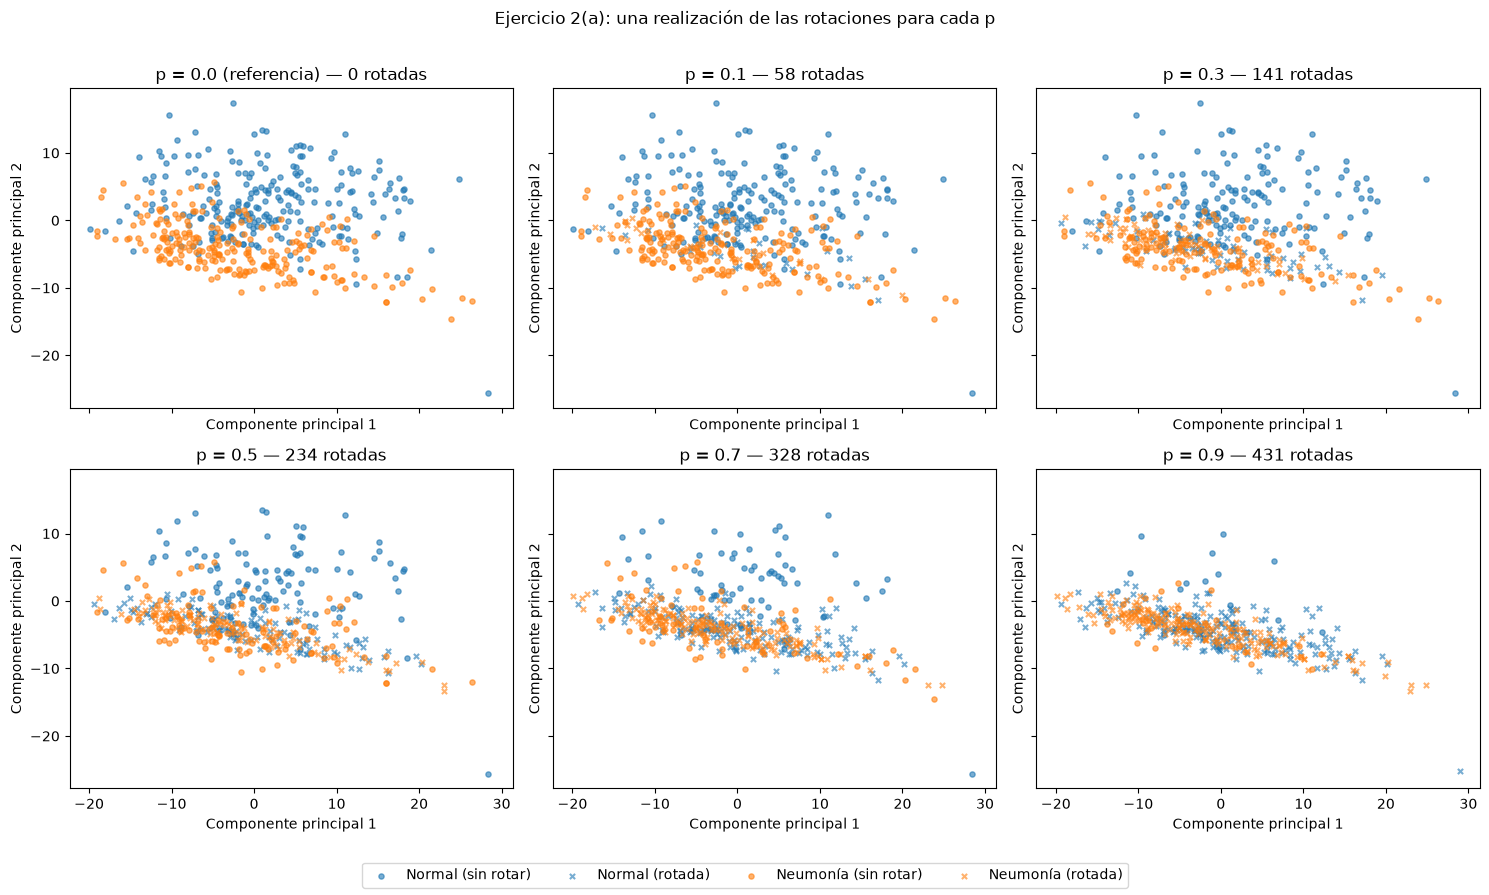
\includegraphics[width=0.86\textwidth]{perturbed_scatter.png}
  \caption{Una realización de las rotaciones para cada $p$, proyectada sobre las dos primeras componentes.
           Círculos: imágenes sin rotar; cruces: imágenes rotadas.}
  \label{fig:pert}
\end{figure}

Nuestra interpretación es la siguiente. Si $R(x)$ es la imagen $x$ rotada, por linealidad se cumple
$R(x)-\mu = R(x-\mu) + \big(R(\mu)-\mu\big)$. El segundo término es igual para todas las imágenes y es
grande, porque en la imagen media rotada los hombros quedan abajo y el diafragma arriba. Al proyectarlo se
obtiene $(-1.7,\,-3.9)$, un desplazamiento común hacia la zona de neumonía. El primer término depende de
cada imagen, pero las direcciones principales se aprendieron con radiografías derechas: la PC2 compara los
pulmones con la periferia, y en una imagen invertida esas zonas quedan desalineadas. Por eso, sobre la PC2
la dispersión se reduce a la mitad (el desvío pasa de 5.6 a 2.8) y la media queda cerca de $-4.2$ para ambas
clases, es decir, se pierde la información de la clase. En cambio, la PC1, que mide el brillo total, casi no
cambia al rotar (la correlación entre la coordenada original y la rotada es 0.99), y por eso la franja
conserva su ancho horizontal. Como consecuencia, al rotar todo el conjunto de prueba el 97.4\,\% de las
imágenes se clasifica como neumonía (contra un 57.3\,\% sin rotar). El acierto en la clase Neumonía sube de
0.876 a 0.996, pero en la clase Normal cae de 0.731 a 0.047. El \acc{} con todo el conjunto rotado, al que
llamamos $A_1$, es 0.521, casi el mismo que el del azar.

\subsection{\texorpdfstring{Accuracy medio en función de $p$ (inciso b)}{Accuracy medio en función de p (inciso b)}}

Para cada $p$ estimamos $\E[A_p]$ con el promedio de los 2000 \emph{accuracies} simulados,
\[ \widehat{\E}[A_p] = \frac{1}{N_{MC}}\sum_{i=1}^{N_{MC}} A_{p,i} . \]
La Figura~\ref{fig:mean} muestra que el \acc{} medio disminuye de forma lineal, desde 0.789 para $p=0.05$ hasta 0.550 para $p=0.9$, sin llegar nunca a
0.5. Esta linealidad tiene una explicación sencilla. Sea $c_i^{\text{der}}=1$ si la imagen $i$ se clasifica
bien cuando está derecha (y 0 si no), y $c_i^{\text{rot}}$ lo mismo cuando está rotada. Como la imagen se
rota con probabilidad $p$, la probabilidad de acertarla es $(1-p)\,c_i^{\text{der}} + p\,c_i^{\text{rot}}$.
Promediando sobre las 468 imágenes, por linealidad de la esperanza se obtiene
\[ \E[A_p] = (1-p)\,A_0 + p\,A_1 \approx 0.803 - 0.282\,p . \]
La Tabla~\ref{tab:mc} compara las estimaciones de Monte Carlo con esta recta. Las diferencias no superan
0.0004 para ninguno de los 18 valores de $p$, lo que funciona como una verificación independiente de la
simulación.

\begin{figure}[H]
  \centering
  \begin{minipage}[t]{0.54\textwidth}\vspace{0pt}
    \centering
    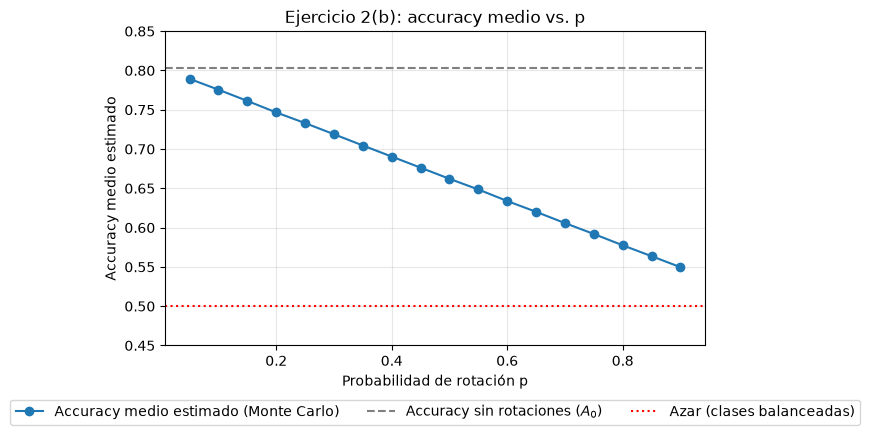
\includegraphics[height=4.4cm]{expected_accuracy_vs_p.png}
    \caption{\emph{Accuracy} medio estimado en función de $p$, junto con $A_0$ (discontinua) y el azar
             (punteada).}
    \label{fig:mean}
  \end{minipage}\hfill
  \begin{minipage}[t]{0.43\textwidth}\vspace{0pt}
    \centering
    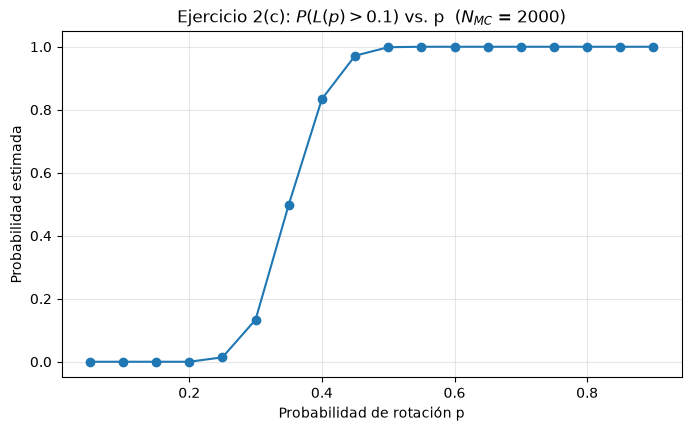
\includegraphics[height=4.4cm]{loss_probability_vs_p.png}
    \caption{Probabilidad estimada de que la pérdida supere $\delta = 0.1$, en función de $p$.}
    \label{fig:prob}
  \end{minipage}
\end{figure}

\begin{table}[H]
  \centering
  \caption{Resultados de Monte Carlo ($N_{MC}=2000$) para algunos valores de $p$: \emph{accuracy} medio
           estimado, valor de la recta $(1-p)A_0+pA_1$, desvío estándar de $A_p$ y probabilidad estimada de
           que la pérdida supere 0.1.}
  \label{tab:mc}
  \small
  \setlength{\tabcolsep}{4.5pt}
  \begin{tabular}{lcccccccccc}
    \toprule
    $p$ & 0.10 & 0.20 & 0.25 & 0.30 & 0.35 & 0.40 & 0.45 & 0.50 & 0.70 & 0.90 \\
    \midrule
    $\widehat{\E}[A_p]$           & 0.7755 & 0.7466 & 0.7330 & 0.7188 & 0.7045 & 0.6904 & 0.6763 & 0.6621 & 0.6057 & 0.5496 \\
    $(1-p)A_0+pA_1$               & 0.7752 & 0.7470 & 0.7329 & 0.7188 & 0.7047 & 0.6906 & 0.6765 & 0.6624 & 0.6060 & 0.5496 \\
    Desvío de $A_p$               & 0.0088 & 0.0118 & 0.0129 & 0.0133 & 0.0144 & 0.0145 & 0.0145 & 0.0150 & 0.0134 & 0.0088 \\
    $\widehat{\Prob}_p(L(p)>0.1)$ & 0.0000 & 0.0000 & 0.0140 & 0.1335 & 0.4985 & 0.8340 & 0.9715 & 0.9985 & 1.0000 & 1.0000 \\
    \bottomrule
  \end{tabular}
\end{table}

\subsection{Probabilidad de que la pérdida supere la tolerancia (inciso c)}

Estimamos $\Prob_p(L(p)>\delta)$, con $\delta=0.1$, como la proporción de simulaciones en las que la pérdida
superó la tolerancia:
\[ \widehat{\Prob}_p\big(L(p)>\delta\big) = \frac{1}{N_{MC}}\sum_{i=1}^{N_{MC}}\ind\{L_i(p)>\delta\} . \]
La condición $L(p)>0.1$ equivale a obtener como máximo 329 aciertos, es decir, al menos 47 menos que sin
rotaciones. La curva de la Figura~\ref{fig:prob} tiene forma de S. Para $p\le0.20$ ninguna de las 2000
simulaciones superó la tolerancia; entre $p=0.25$ y $p=0.45$ la probabilidad sube de 0.014 a 0.972, y desde
$p=0.50$ es prácticamente 1. La probabilidad vale aproximadamente $1/2$ cuando el \acc{} medio coincide con el
umbral $A_0-\delta$. Según la recta anterior, esto ocurre en $p^*=\delta/(A_0-A_1)=0.1/0.282\approx0.355$, lo
que coincide con el 0.4985 estimado para $p=0.35$. El cambio es brusco porque el \acc{} de cada realización
se aleja poco de su media (su desvío es de a lo sumo 0.015): si la media está a dos o tres desvíos del
umbral, casi ninguna simulación lo cruza, o lo cruzan casi todas. En la práctica, el sistema tolera hasta un
20--25\,\% de imágenes rotadas sin que la pérdida supere 0.1, pero con un 45\,\% la supera casi siempre.

\subsection{Distribución del accuracy (inciso d)}

La Figura~\ref{fig:hist} muestra los histogramas de los 2000 \emph{accuracies} para cada $p$. Como el \acc{}
solo toma valores de la forma $k/468$, usamos un intervalo centrado en cada valor posible, con ancho $1/468$.
Así evitamos que algunos intervalos agrupen dos valores posibles y otros queden vacíos, lo que generaría
huecos artificiales. Las distribuciones tienen forma de campana y están centradas en la media estimada, que
se desplaza hacia la izquierda al crecer $p$. Su ancho es máximo en $p=0.5$ y simétrico alrededor de ese
valor: el desvío es 0.009, 0.013, 0.015, 0.013 y 0.009 para $p = 0.1$, $0.3$, $0.5$, $0.7$ y $0.9$. Esto se
explica con el mismo razonamiento del inciso (b). Solo influyen las 188 imágenes cuya clasificación cambia al
rotarlas (160 pasan de acierto a error y 28 de error a acierto), y cada una se rota de forma independiente
con probabilidad $p$, por lo que
\[ \operatorname{Var}(A_p) = \frac{188\,p\,(1-p)}{468^2}, \]
que es máxima en $p=0.5$ y toma el mismo valor en $p$ y en $1-p$. Para $p=0.5$ la fórmula da un desvío de
0.0146, muy cercano al 0.0150 observado. La forma de campana se debe a que $A_p$ es una suma de muchas
contribuciones independientes, situación en la que el Teorema Central del Límite indica que la distribución
se aproxima a una normal.

\begin{figure}[H]
  \centering
  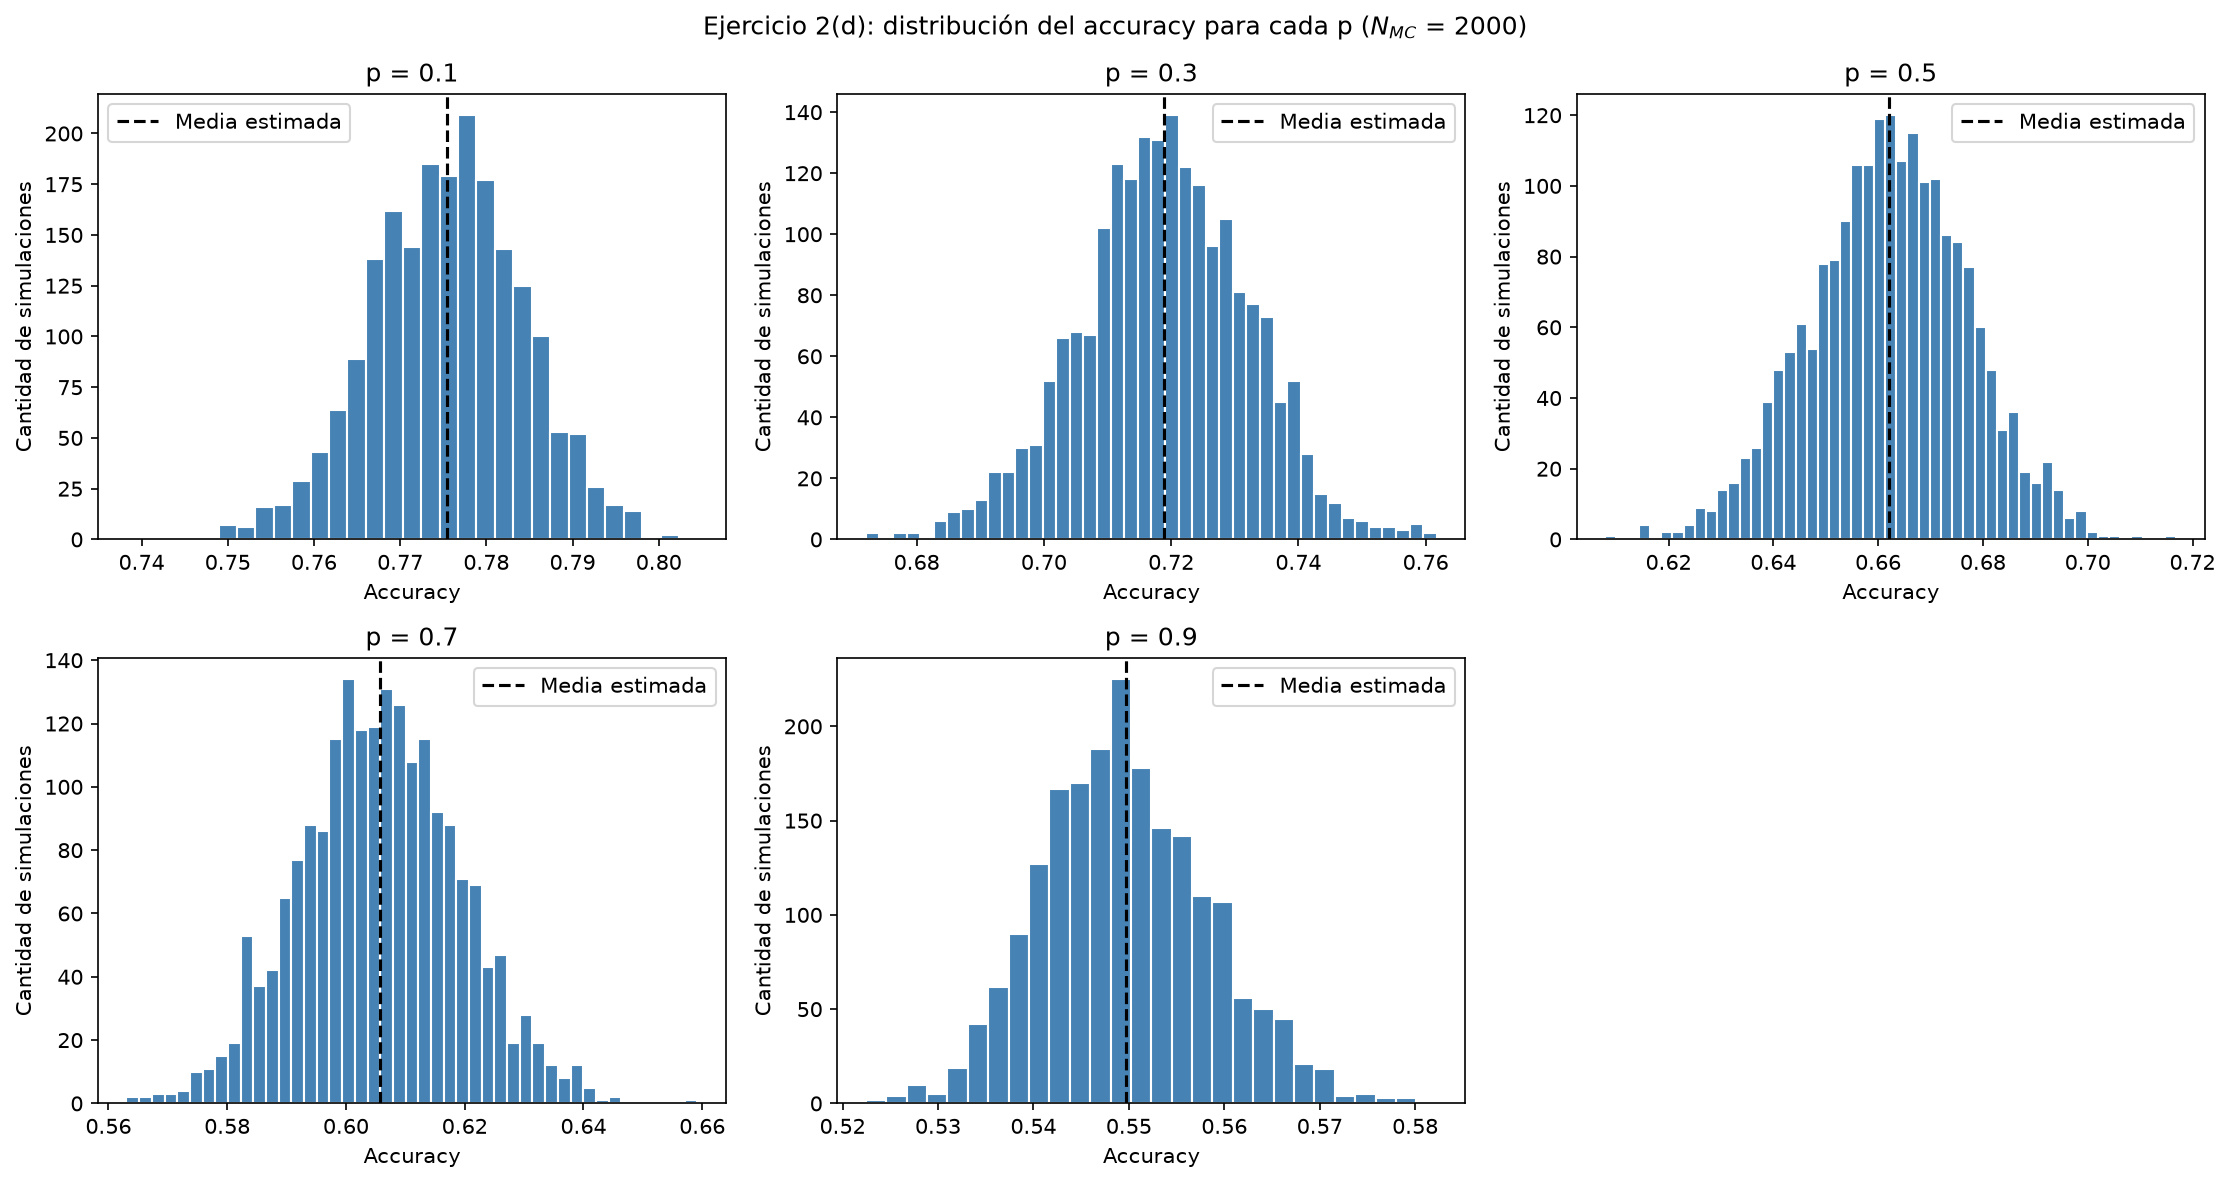
\includegraphics[width=0.86\textwidth]{accuracy_histograms.png}
  \caption{Histogramas del \emph{accuracy} en las 2000 simulaciones para cada $p$. La línea punteada indica
           la media estimada.}
  \label{fig:hist}
\end{figure}

\subsection{Estabilidad de las estimaciones}

La Figura~\ref{fig:conv} muestra, para $p=0.35$, cómo evolucionan las dos estimaciones al acumular
simulaciones. Elegimos este valor porque la probabilidad buscada está cerca de 0.5, que es el caso de mayor
varianza de la indicadora y, por lo tanto, el más difícil de estimar. Al principio las estimaciones cambian
bruscamente (con una sola simulación, la probabilidad solo puede valer 0 o 1), pero luego se estabilizan: la
probabilidad queda cerca de 0.50 desde unas 300 simulaciones, y el \acc{} medio queda alrededor de 0.7045
desde unas 1000. Este es el comportamiento que predice la Ley de los Grandes Números.

\begin{figure}[H]
  \centering
  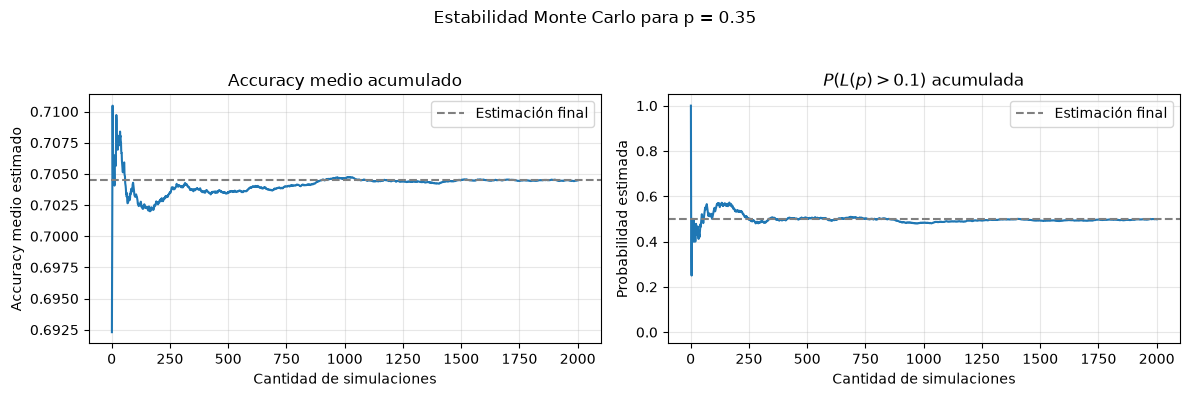
\includegraphics[width=0.84\textwidth]{monte_carlo_convergence.png}
  \caption{Evolución de las estimaciones para $p = 0.35$ según la cantidad de simulaciones acumuladas.
           Izquierda: \emph{accuracy} medio. Derecha: probabilidad de que la pérdida supere 0.1.}
  \label{fig:conv}
\end{figure}

% =====================================================================
\section{Ejercicio 3: justificación mediante la Ley de los Grandes Números}
\label{sec:ej3}
% =====================================================================
Fijado $p$, en cada simulación se hace un sorteo nuevo e independiente de las rotaciones, mientras que el
modelo, el conjunto de prueba y $A_0$ no cambian. Por lo tanto, $A_{p,1},\dots,A_{p,N}$ son variables
independientes e idénticamente distribuidas (i.i.d.), con la misma distribución que $A_p$, y lo mismo vale
para las pérdidas $L_i(p)=A_0-A_{p,i}$. Como es habitual, suponemos que los números pseudoaleatorios de la
computadora se comportan como sorteos independientes. Definimos $X_i=\ind\{L_i(p)>\delta\}$, que vale 1 si en
la simulación $i$ la pérdida supera $\delta$, y 0 si no. Las $X_i$ son i.i.d. y tienen distribución de
Bernoulli con parámetro $q=\Prob_p(L(p)>\delta)$, que es justamente la probabilidad que queremos estimar:
\[
  \E[X_i] = 1\cdot\Prob\big(L_i(p)>\delta\big) + 0\cdot\Prob\big(L_i(p)\le\delta\big) = q,
  \qquad \operatorname{Var}(X_i) = q(1-q) \le \tfrac14 .
\]
El estimador es el promedio muestral
\[ \hat q_N = \frac1N\sum_{i=1}^N X_i = \frac1N\sum_{i=1}^N \ind\{L_i(p)>\delta\}, \]
es decir, la proporción de simulaciones en las que ocurrió el evento. Por linealidad de la esperanza y por la independencia de las $X_i$,
\[
  \E[\hat q_N] = q, \qquad \operatorname{Var}(\hat q_N) = \frac{q(1-q)}{N},
\]
así que el estimador es insesgado y su varianza disminuye al aumentar $N$. La Ley Débil de los Grandes
Números~\cite{leongarcia,teoricas} asegura que el promedio de variables i.i.d. con media y varianza finitas
converge en probabilidad a esa media. En este caso podemos verlo directamente con la desigualdad de Chebyshev:
para todo $\varepsilon>0$,
\[
  \Prob\big(|\hat q_N - q|\ge\varepsilon\big) \le \frac{\operatorname{Var}(\hat q_N)}{\varepsilon^2}
  = \frac{q(1-q)}{N\varepsilon^2} \le \frac{1}{4N\varepsilon^2} \xrightarrow[N\to\infty]{} 0 .
\]
Es decir, con suficientes simulaciones, la probabilidad de que la proporción observada se aleje de la
probabilidad verdadera en más de $\varepsilon$ es tan pequeña como se quiera. Esto justifica estimar
$\Prob_p(L(p)>\delta)$ como el promedio de las funciones indicadoras. La Ley Fuerte agrega que $\hat q_N$
converge a $q$ con probabilidad 1, que es lo que se observa en la Figura~\ref{fig:conv}. Con $N_{MC}=2000$, la
cota da un desvío de a lo sumo $1/\sqrt{8000}\approx0.011$ y garantiza que
$\Prob(|\hat q_N-q|\ge0.05)\le 1/(8000\cdot 0.05^2) = 0.05$. Esta cota es conservadora porque corresponde al
peor caso, $q=0.5$. El mismo argumento vale para el estimador de $\E[A_p]$: los $A_{p,i}$ son i.i.d. y toman
valores entre 0 y 1, por lo que su varianza es finita y su promedio converge a $\E[A_p]$. La coincidencia con
la fórmula exacta en la Tabla~\ref{tab:mc} muestra esta convergencia en la práctica.

% =====================================================================
\section{Conclusiones}
% =====================================================================
PCA permitió reducir drásticamente la dimensión de las radiografías sin perder capacidad de clasificación.
Con 3 componentes se igualó el \acc{} de la imagen completa (0.818) y con 5 se llegó a 0.857, posiblemente
porque un modelo con menos entradas tiene menos riesgo de sobreajuste. También vimos que PCA ordena las
direcciones por varianza y no por su utilidad para clasificar: la PC1 mide el brillo general y casi no separa
las clases, mientras que la PC2, relacionada con la opacidad de los pulmones, es la que las distingue.
Además, conservar el 90\,\% de la varianza habría requerido 121 componentes, muchas más de las necesarias.

El sistema PCA+LR resultó poco robusto frente a rotaciones de 180°. Las imágenes rotadas caen en la región
asociada a la neumonía y, con todo el conjunto rotado, el \acc{} baja a 0.521. Con Monte Carlo estimamos que
el \acc{} medio disminuye linealmente con $p$ y que la probabilidad de perder más de 0.1 pasa de casi 0 a casi
1 entre $p=0.25$ y $p=0.45$. Las estimaciones coincidieron con las fórmulas que dedujimos para la media y la
varianza del \acc{}. Por su parte, los gráficos de estabilidad y la cota de Chebyshev ilustraron en la
práctica la Ley de los Grandes Números.

Las principales dificultades que encontramos, y la forma en que las resolvimos, fueron:
\begin{itemize}
  \item \textbf{Tamaño de los datos:} la matriz de covarianza de $16384\times16384$ era demasiado grande, así
        que calculamos PCA con la SVD reducida de la matriz centrada, una sola vez para todos los $K$.
  \item \textbf{Proyección del conjunto de prueba:} entendimos que $U_KS_K$ solo vale para las imágenes de
        entrenamiento, y que las de prueba deben proyectarse con $(X-\mu)V_K$, usando la media y las
        direcciones de entrenamiento.
  \item \textbf{Cantidad de cálculo en las simulaciones:} en lugar de rotar, proyectar y clasificar el
        conjunto de prueba en cada una de las 36000 realizaciones, precalculamos las dos predicciones
        posibles de cada imagen y verificamos que el resultado fuera idéntico.
  \item \textbf{Interpretación de los resultados:} para darles sentido a los ejes de PCA graficamos las
        componentes como imágenes y calculamos el cociente de Fisher. Además, tuvimos en cuenta que, con
        468 imágenes de prueba, una diferencia de 0.01 equivale a unas 5 imágenes.
\end{itemize}

% =====================================================================
{\small
\begin{thebibliography}{9}
\bibitem{mahmood} Mahmood, B. (2016). \emph{How to Predict Yes/No Outcomes Using Logistic Regression}.
  Medium.
\bibitem{medmnist} Yang, J. et al. (2024). \emph{MedMNIST+}: PneumoniaMNIST ($128\times128$).
\bibitem{leongarcia} Leon-Garcia, A. (2008). \emph{Probability, Statistics, and Random Processes for
  Electrical Engineering} (3.ª ed.). Pearson Prentice Hall.
\bibitem{teoricas} Material teórico de I206 -- Inferencia y Estimación (2026): \emph{Análisis de componentes
  principales} y \emph{Convergencia -- Monte Carlo}. Universidad de San Andrés.
\bibitem{sklearn} Pedregosa, F. et al. (2011). Scikit-learn: Machine Learning in Python.
  \emph{Journal of Machine Learning Research}, 12, 2825--2830.
\bibitem{numpy} Harris, C. R. et al. (2020). Array programming with NumPy. \emph{Nature}, 585, 357--362.
\end{thebibliography}
}

\end{document}
